% IEEE standard conference template; to be used with:
%   spconf.sty  - LaTeX style file, and
%   IEEEbib.bst - IEEE bibliography style file.
% --------------------------------------------------------------------------

\documentclass[letterpaper]{article}
\usepackage{spconf,amsmath,amssymb,graphicx}
\usepackage{multicol, hyperref}
\usepackage{todonotes}
\usepackage[linesnumbered]{algorithm2e}
\usepackage{enumitem}
\usepackage{capt-of}
\usepackage[skip=0pt]{caption}

% Example definitions.
% --------------------
% nice symbols for real and complex numbers
\newcommand{\R}[0]{\mathbb{R}}
\newcommand{\C}[0]{\mathbb{C}}

% bold paragraph titles
\newcommand{\mypar}[1]{{\bf #1.}}


% Title.
% ------
\title{Fast 2D $N^2$ t-distributed Stochastic Neighbor Embedding}
%
% Single address.
% ---------------
\name{Marc Fischer, Alberto Montes, Marko Pichler Trauber, Andreas Bl\"ochliger}
\address{Department of Computer Science\\ ETH Z\"urich\\Z\"urich, Switzerland}

% For example:
% ------------
%\address{School\\
%		 Department\\
%		 Address}
%
% Two addresses (uncomment and modify for two-address case).
% ----------------------------------------------------------
%\twoauthors
%  {A. Author-one, B. Author-two\sthanks{Thanks to XYZ agency for funding.}}
%		 {School A-B\\
%		 Department A-B\\
%		 Address A-B}
%  {C. Author-three, D. Author-four\sthanks{The fourth author performed the work
%		 while at ...}}
%		 {School C-D\\
%		 Department C-D\\
%		 Address C-D}
%

\begin{document}
%\ninept
%
\maketitle
%

\begin{abstract}
We present a faster implementation of the $N^2$ t-SNE embedding. Our version is restricted to producing 2D output vectors and developed for CPU architectures supporting AVX2 instructions. We analyze performance blockers and elevate them by increasing locality and hand-optimizing the code. This yields the fastest implementation known to the authors.
\end{abstract}

\section{Introduction}\label{sec:intro}

\mypar{Motivation} It's difficult to understand today's increasingly huge and high-dimensional datasets. Different forms manifold learning, dimension reduction and embedding algorithms can be employed to aid in this. They transform high dimensional datasets into lower dimensional ones, while preserving certain characteristics of the data. This can be used to obtain input data of a certain dimensionality, e.g. as input for further algorithms or for visualization in 2 or 3 dimensions.

t-distributed Stochastic Neighbor Embedding (t-SNE) is a recent \cite{maaten_visualizing_2008, van_der_maaten_accelerating_2014} algorithm mainly used for such visualizations. Speeding up t-SNE, leads to much faster feedback as well as the possibility to apply it to larger datasets.

While the algorithm has a lot of independent computations, a fast implementation is hard to achieve. Those parts are well suited for parallelism. While we focus on a single-thread implementation, this still allows easy usage of ILP and vectorization. A big problem is that it is usually applied to large and high dimensional data sets, which can lead to bad data locality, impacting the performance.
Another performance blocker is in the structure of the computation. Many values need normalized by the sum of all related values. This means looping through the same data twice, resulting in bad locality if the data is larger than the cache.

There are two versions of the algorithm. An exact one, the $N^2$ version, and an approximate $N \log N$ version. For further discussion see Section~\ref{sec:background}.

In this work we present a fast implementation for the $N^2$ version. Our implementation is not restricted in the input dimension $D$ or the number of input vectors $N$, but we generally consider cases for $D < 5000$ and $N < 10000$. However we restrict the output dimension to $d=2$, which is by far the most important application for t-SNE. For those restrictions our implementation is faster than comparable implementations. Our approach is flexible in the number of iterations $T$ and perplexity $P$, but we consider $T= 1000$ and $P = 50$, which are common choices.

\mypar{Related work}
The openly available implementations of the algorithm are curated\footnote{\url{https://lvdmaaten.github.io/tsne/\#implementations}} by the author of the algorithm \cite{maaten_visualizing_2008, van_der_maaten_accelerating_2014}. Some are "fast" in different senses, i.e. a CUDA version, making use of parallelism and some implement the $N \log N$ version. The default C++ version claims to be the "fastest" available. This seems plausible in terms of run time as it seems to be the only serious C++ implementation and also since it implements both versions. The implementation is solid, clean and certainly not slow C++ code, but it is also clearly not specifically optimized for performance or runtime.
Our approach builds on this code-base. Our baseline version is an adjusted and highly instrumented version of this implementation. Thus whenever we refer to the "baseline" performance in this work it can be considered a comparison to this implementation.

\section{Background: The t-SNE Algorithm}\label{sec:background}

\begin{figure*}[h]
\begin{minipage}{0.63\hsize}
\begin{algorithm}[h] \footnotesize
 \KwData{high dimensional data $\mathbf{X} = \{\mathbf{x}_1, \dots, \mathbf{x}_N \} \subseteq \mathbb{R}^D$, Target Perplexity $P$, Number of iterations $T$}
 \KwResult{low dimensional data $\mathbf{Y} = \{\mathbf{y}_1, \dots, \mathbf{y}_N \} \subseteq \mathbb{R}^d$ such that $d \ll D$} %(usually d = 2 or 3)}
 	subtract mean $\forall i = 0..N \quad \mathbf{x}_i = \mathbf{x}_i - \bar{\mathbf{x}}$\;
 	rescale data $\forall i = 0..N, \, k = 0..D \quad \left(\mathbf{x}_i\right)_k = \left(\mathbf{x}_i\right)_k / \max_{i', k'} \left(\mathbf{x}_{i'}\right)_{k'}$\;
	compute squared euclidean distances $d_{ij} = \| \mathbf{x}_i - \mathbf{x}_j \|^2$ \;
	\For{$i = 0 .. N$}{
		initialize $\sigma_i$\;
		\Repeat{$\text{per}_i \approx P$}{
			$\forall j = 0..N \quad p_{j|i} = \frac{ \exp(- d_{ij} / 2 \sigma^2_i ) }{ \sum_{k \neq i } \exp(- d_{ik} / 2 \sigma^2_i )}$\;
			$\text{per}_i = 2^{\sum_j p_{j|i} \log_2 p_{j|i}  }$\;
		}
	}
	symmetrize and normalize affinities $\forall i,j = 0..N \quad p_{ij} = \frac{p_{j|i} + p_{i|j}}{2N}, \quad p_{ij} = p_{ij} / \sum_{i,j} p_{ij}$ \;
% 	normalize affinities $\forall i,j = 0..N p_{ij} = p_{ij} / \sum_{i,j} p_{ij}$ \;
	sample initial $\mathbf{Y}^{(0)} = \{\mathbf{y}_1^{(0)}, \dots, \mathbf{y}_N^{(0)} \}$ from Gaussian distribution\;
	\For{$t = 1 .. T$}{
		$\forall i,j = 0..N \quad t_{ij} =  (1 + \| \mathbf{y}_i^{(t-1)} - \mathbf{y}_j^{(t-1)} \|^2)^{-1} \quad T =  \sum_{k \neq l} t_{kl} $\;
		compute $\forall i = 0..N \quad  \frac{\partial C}{\partial \mathbf{y}_i^{(t-1)}} = 4 \sum_j (p_{ij} - \frac{t_{ij}}{T}) (\mathbf{y}_i^{(t-1)} - \mathbf{y}_j^{(t-1)}) t_{ij}$\;
		update $\forall i = 0..N \quad  \mathbf{y}_i^{(t)} = \mathbf{y}_i^{(t-1)} + \eta \frac{\partial C}{\partial \mathbf{y}_i^{(t-1)}} + \alpha(t) (\mathbf{y}_i^{(t-1)} - \mathbf{y}_i^{(t-2)}) $ \;
		subtract mean $\forall i = 0..N \quad \mathbf{y}_i^{(t-1)} = \mathbf{y}_i^{(t-1)} - \bar{\mathbf{y}}^{(t-1)}$\;
	}

    \caption{tSNE Algorithm}
    \label{algo:tSNE}
\end{algorithm}
\end{minipage}
\hfill
{
\begin{minipage}{0.33\hsize}
    \centering
    \resizebox{\textwidth}{!}{
    \begin{tabular}{|l|c|c|c|}
     \hline
                & \textbf{Part 1} & \textbf{Part 2} & \textbf{Part 3}\\ \hline
        add     & $DN^2$    & $(3N^2 + 4NI)/2$  & $TN^2d$\\ \hline
        mult    & $DN^2 /2$ & $N^2 + 3NI$       & $TN^2d / 2$\\ \hline
        div     & $DN$      & $2N^2 + 2 I$      & $(TN^2 + TNd)/2$\\ \hline
        exp     &           & $NI$              & \\ \hline
        log     &           & $2I$              & \\ \hline
    \end{tabular}
    }
    \captionof{table}{Leading term of the cost for each part. Other terms and constants omitted for reasons of space.}
    \label{tab:cost}
    \vspace{10mm}
    \resizebox{\textwidth}{!}{
    \begin{tabular}{|l|r|r|r|}
        \hline
                & $D = 500$ & $D = 1000$    & $D = 2500$\\ \hline
        Part 1  & 4.49 \%    & 8.84 \%  & 23.33 \% \\ \hline
        Part 2  & 18.06 \%   & 17.24 \% & 17.28 \% \\ \hline
        Part 3  & 77.45 \%   & 73.92 \% & 59.39 \% \\ \hline
    \end{tabular}
    }
    \captionof{table}{Breakdown of cycles for N = 1000, varying D for randomly generated input data. For growing D, Part 1 becomes more and more a bottleneck.}
    \label{tab:breakdown}
\end{minipage}
}
\vspace{-5mm}
\end{figure*}

\mypar{t-SNE Algorithm, Algorithmic Cost}
A simplified version of the algorithm as we implement it is given in Algorithm~\ref{algo:tSNE}. The literature distinguishes two versions of the algorithm. The presented version has asymptotic runtime in $O(N^2)$, which can be seen easily as quantities such as $q_{ij}$ or $p_{i|j}$ are calculated for all $i$-$j$ pairs. The other version constructs trees (based on quadtrees), which allow to easily find the nearest neighbors for each data point. The pairwise quantities, such as $p_{i|j}$ and $q_{ij}$ are only calculated for those nearest neighbors. This version is dominated by creating and searching the trees and thus has asymptotic runtime $O(N \log N)$. For very large inputs $N > 10000$ the second version is usually faster. Many of the optimizations discussed here, should also be applicable to the $N \log N$ version, as the algorithms share a lot of their structure. The main challenge is likely to store the trees in an array like structure with some locality, i.e. by using Z order curves \cite{stann_nearest} as well as through thorough analysis of the algorithm to avoid recreation and reordering of the trees. Since this is more of an algorithmic problem, we did not address it here.

\mypar{Cost Analysis}
While our implementation generally uses the structure in Algorithm~\ref{algo:tSNE}, some optimization can already be made here. The power of 2 in line 8 can be avoided by taking the logarithm of both sides and computations such as the squared euclidean distances have symmetry. Optimization of that sort where already implemented in the baseline.

In our performance measurements we computed the flops exactly and used the following cost measure $Cost(N, D, d) = (\# \text{adds}, \# \text{mults}, \# \text{divs}, \# \text{exps}, \# \text{logs})$.

We divided the code in 3 rough parts, which were optimized independently. Part 1 comprises lines 1-3, the prepossessing and calculation of the squared euclidean distance in high dimension D. Part 2 is the calculation of the high dimensional affinities, lines 4-12. The last part is the main loop on lines 13 to 19. Table~\ref{tab:cost} shows the leading term of the cost measure.

Part 2 depends on $I$, the total number of iterations of the inner loop (lines 6-9 in the algorithm). In our measurements we have seen that on average the loop iterates 20 times for each point. Thus $I \approx 20 N$ works well for back-of-the-envelope calculations. For actual performance calculations we run the program twice. In the first run we count the actual iterations $I$, the second time we run the program without that counter to obtain the runtime in cycles.

\section{Fast Implementation}\label{sec:fastImplementation}

Table~\ref{tab:breakdown} shows the breakdown of the runtime spend in the different parts. Part 3 is the most expensive part, as it is executed $T \approx 1000$ times. However also Part 1 can profit from optimization. It is the only part for which the costs depends on the input dimension. Thus for larger $D$ it becomes more of a performance blocker than for lower $D$. This leaves parts 1 and 3 as obvious targets for optimization. We also invested some optimization in part 2, but it is not critical for the overall performance.


\subsection{Part 1: Reprocessing \& Euclidean Distance}

Part 1 consists of two smaller steps: normalizing the data and computing the euclidean distance.

\mypar{Structure, Loop Fusion}
In the baseline this is implemented in 5 distinct loops over the data; calculate mean, subtract mean, find maximum, divide by maximum, calculate euclidean distances.
It is obvious that this had bad locality if the working set is larger than the cache (which is likely for large N and D).

Loop fusion allows to write the program with 2 loops: calculate mean, subtract mean and calculate maximum in the first loop; calculate euclidean distance and apply scaling the second. Since we need the mean in order to subtract it we can not fully fuse the loops, and obtain the following structure:


\begin{algorithm} \footnotesize
    maxX = 0 \;
	\For{k =0:D}{
    	\For{i=0:N}{
    	    mean[k] += X[i][k] \;
    	}
    	mean[k] /= N \;
    	\For{i=0:N}{
    	    $\mathbf{X}$[i][k] -= mean[k] \;
    	    maxX = max(maxX, abs($\mathbf{X}$[i][k])) \;
    	}
	}
	\For{i=0:N}{
	    for all j calculate $d_{ij}$
	}
\end{algorithm}


Unrolling the outer loop in k, i.e. by 8, allows to use multiple accumulators and since only 8 dimensions are accessed at once, even for N = 10000 the working set (all relevant parts of $\mathbf{X}$ and means) are in cache (L2 or L3). Thus the second inner loop has temporal locality on the $\mathbf{X}$ and means. And since we access 8 continuous floats a time we also have spatial locality in the inner loops. Since data is likely not perfectly aligned this might actually be two cache lines, but the argument stands.
This already concludes the optimization for the prepossessing. This loop can be further improved by hand-vectorizing the code, but this is only a noticeable improvement for very low N as the cost for the euclidean distance dominates Part 1.

\mypar{High Dimensional Squared Euclidean Distance}
The second - and much more expensive - step of Part 1 is the calculation of pairwise squared euclidean distance. With the structure: \texttt{for i=1:N} \texttt{\{ for j=i+1:N} \texttt{\{ for k=0:D \} \}}.
Unrolling the innermost loop allows to use multiple accumulators.

A notable piece of strength reduction is the division by N in the first loop and the scaling by the maximum (line 2 in the algorithm). Instead of scaling both $\mathbf{x}$ vectors we can just scale the resulting norm by $\frac{1}{\text{maxX}^2}$. Interestingly we observed that this is in most cases numerically \textit{more} stable for this application. We can precompute $\frac{1}{\text{maxX}^2}$ after the first loop over D and also $\frac{1}{N}$ in the beginning, thus turning all divisions into multiplications.

Along with further strength reduction, single static assignment, scalar replacement and sharing common subexpressions this concludes the basic scalar version. In Figure~\ref{fig:part1:novec} this is called "Fast Scalar".

\begin{figure}[h]
  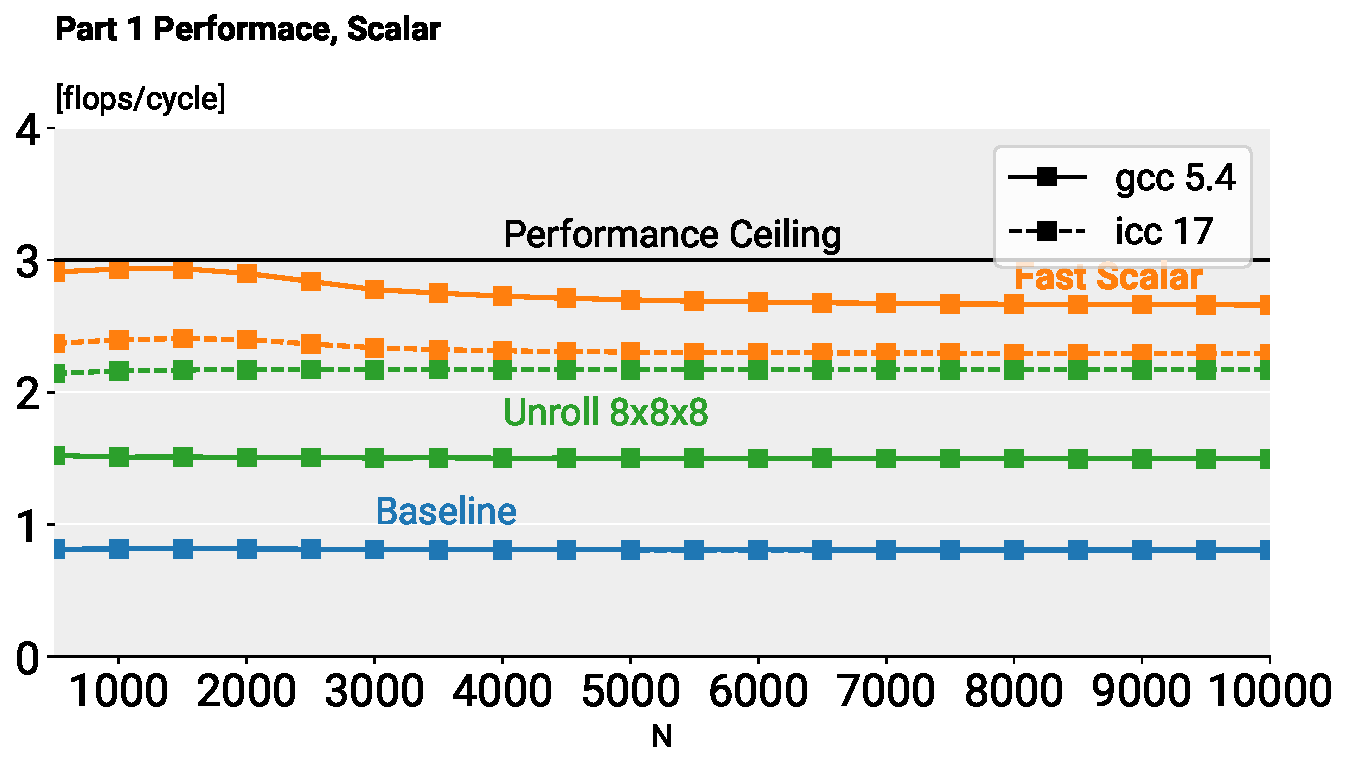
\includegraphics[width=\linewidth]{images/part1_novec}
  \caption{Performance for part 1. No autovectorization. For details about the setup see section~\ref{sec:exp}.}
   \label{fig:part1:novec}
   \vspace{-5mm}
\end{figure}

\mypar{More unrolling \& Blocking}
To further improve the performance, we can block the loops over $i,j$. We blocked have the outer loops by a factor 8 and unrolled the inner loop by factor 8. This allows to access data in the result matrix (each entry $i,j$ is the euclidean distance of $\mathbf{x}_i, \mathbf{x}_j$) in $8 \times 8$ blocks. We can compute one $8\times 8$ block, store it and store it in it's transposed position. Since we are using $8 \times 8$ blocks, even the transposed store should be cheap, as we will be fully using all the cache lines. We also fully unroll the inner the loop in j.
In \texttt{gcc} this is actually quite bad. Either because this coding style does not allow as many compiler optimization (automatic loop optimization) or because  the working register set is too large (vTune asserts "high register pressure" here). In Figure~\ref{fig:part1:novec} this is called "Unroll 8x8x8".

Without vectorization \texttt{icc} is also a bit worse on this, however, \texttt{icc} is able to auto-vectorize this better than the previous scalar version. Autovectorized results can be see in Figure~\ref{fig:part1:vec}.

\mypar{Hand-Vectorization}
The structure that we obtained from the last optimization step is almost perfect for vectorization. We can use 8 AVX accumulators and in each loop iteration compute for 8 continuous dimensions of 8 $x_j$ vectors. In the end we want to reduce this into one 8 dimensional accumulator. 8 AVX registers are optimal in this case, as it allows a perfect reduction tree for horizontal adds. Figure~\ref{fig:part1:vec} shows the results for this ("AVX") along with the autovectorized versions of the scalar versions.

\begin{figure}[h]
  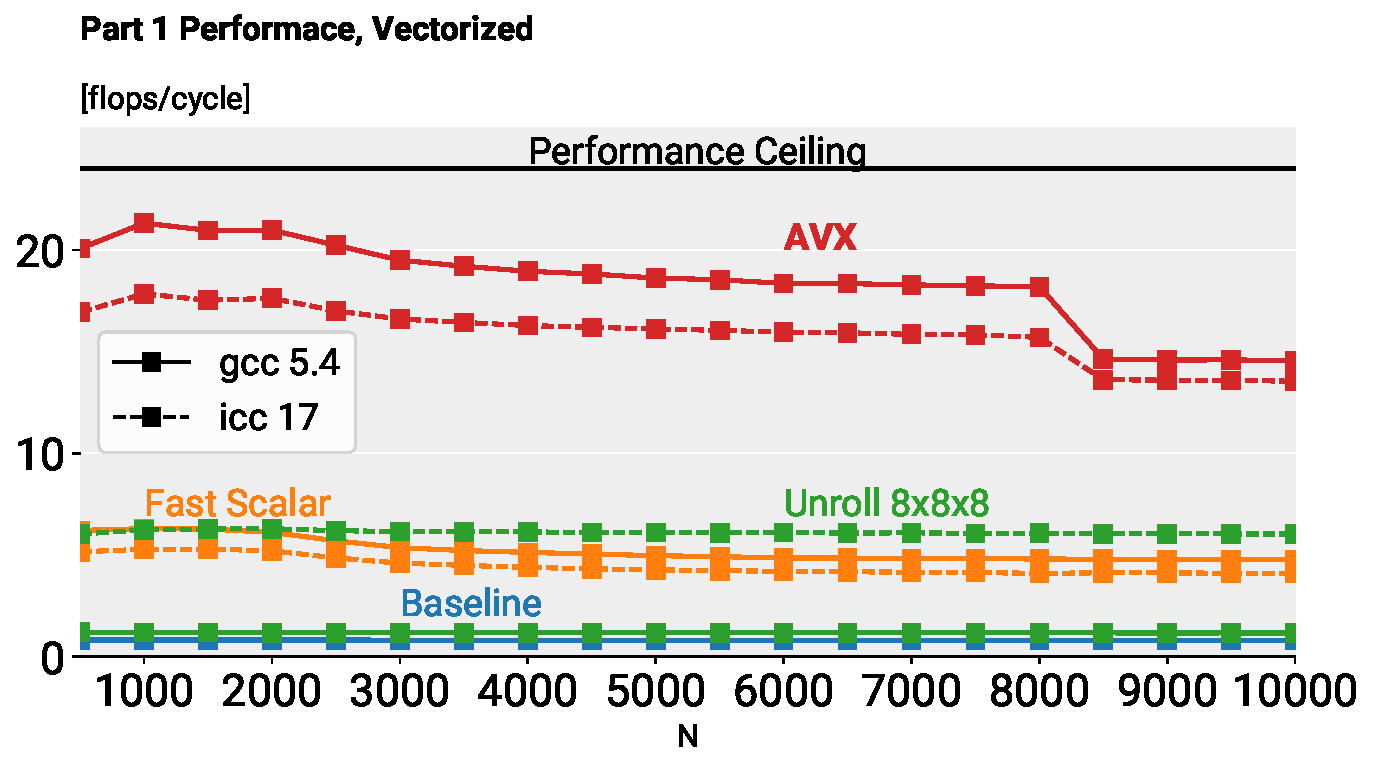
\includegraphics[width=\linewidth]{images/part1_vec}
  \caption{Performance for Part 1. Scalar code was autovectorized. For details about the setup see section~\ref{sec:exp}.}
   \label{fig:part1:vec}
   \vspace{-3mm}
\end{figure}

\mypar{Performance Ceiling}
The computationally most intense part is the inner loop in the euclidean distance. Per iteration we perform 1 subtraction, 1 multiplication, 1 addition. This can be reshaped into a 1 subtraction and 1 FMA per loop iteration. So on a Skylake architecture we could achieve up to $3$ flops/cycle in the scalar case and $24$ flops/cycle in the vectorized case. Outside this loop we have a less favorable instruction mix, so the peak performance is likely a bit lower.

\mypar{What we did not attempt} Since we have seen that scalar performance is actually worse for the blocked/unrolled version, this likely means 2-level blocking would have helped. However since the optimized scalar version and the optimized vectorized version are very close to peak performance, we did not investigate this further.

It should also be stated that, most of the discussed optimizations only work if the relevant dimension is divisible by 8. Thus there is a lot of code for the edge cases, that sometimes uses different unrolling/vectorization schemes and even different loop order.

\mypar{Data loaded \& OI}
The required data in this part is $ND + N^2 + D$ floats. If we assume $D \approx N$ this means that for $N \approx 1000$ the data does not fit into L3 cache anymore. Since most datasets are larger, we will assume $N > 1000$ in our analysis. We need to load \textbf{X} at least 2 times and we need to load and store the resulting distance matrix. Thus $Q(N,D) \geq 4(2 ND +  2N^2)$. This allows us to bound $I(N,D) \leq \frac{3}{16}D + \frac{1}{8} + O(\frac{1}{ND})$.

\subsection{Part 2: High dimensional affinities}
Part 2 computes the pairwise affinities between the high dimensional data points, using the previously computed squared euclidean distances (lines 4-11 in Algorithm~\ref{algo:tSNE}). This requires binary search for optimal variance value $\sigma_i$ around each data point. After we have computed the pairwise affinities, we symmetrize and normalize them.

\mypar{Pairwise Affinities}
We utilized unrolling, accumulators, vectorization and blocking to optimize calculating the pairwise affinities based for a given perplexity. However these approaches did not result in any significant performance improvements.

An issue is that the binary search has a dynamic amount of iterations until the appropriate value is found. Unrolling that loop creates a mismatch between the iterations because of their different duration.
Another problem are the expensive log and exp instructions. Taking their latency into account we calculate a theoretical peak performance $2.21$ flops/cycle. For most versions we measure performance around $1.5$ flops/cycle. We assume that we are actually compute bound (or at least bound by the instruction latency) due to the high number of expensive instructions. Latency hiding is quite involved due to the dynamic inner loop. Since we need one row of the distance matrix for each $i$ other unrolling schemes quickly become memory bound.

We also considered merging this step with the computation with part 1 to reduce memory traffic. However this steps needs a whole row of the input matrix at once, while Part 1 produces them in blocks. While some further optimization schemes might be possible, we did not investigate too much further into them as this step is not a bottleneck.

\mypar{Affinities Symmetrization}
In this step (line 11 in Algorithm~\ref{algo:tSNE}) we want to symmetrize and normalize the previously calculated affinities. We have tried the usual approaches to optimize the code. In the end the best performance was obtained by blocking the matrix access into 8x8 blocks. The access pattern follows a reversed L shaped sequence of blocks and add the blocks and their respective transpose block using a 8x8 AVX transposition macro. While iterating through the data the sum for normalization is computed on the fly. We implement a small extension to the algorithm called "early exaggeration", where the affinities are multiplied with a small constant. This is combined with the normalization in our implementation. This part has not shown to be a bottleneck in the computation before or after optimization. We have achieved roughly four times speedup with the performance of $0.5$-$1.25$ flops/cycle compared to $0.15$-$0.2$ flops/cycle in the base version.

\subsection{Part 3: Training Loop}
The last part of the algorithm (lines 12 - 18 in Algorithm~\ref{algo:tSNE}) computes low dimensional embedding. It randomly initializes a embedding and then for $T$ loop iterations computes the affinities in the embedding space.
Based on the affinities a gradient is computed per point, in order to update it.

\subsubsection{Low Dimensional Affinities}

To compute the low dimensional affinities, the pairwise squared euclidean distance of the $d$-dimensional embedding is computed and an element wise operation is applied (line 14 in the algorithm). We fixed $d=2$.

\mypar{Unrolling and Blocking}
The computation of the low dimensional affinities shares a lot of similarity with the pairwise euclidean distance (part 1). The main difference is that since now the dimensionality is known in advance, allowing easier unrolling and scalar replacement in the inner-most loop, which computes the distance between points. Blocking was implemented for this computation. As with the high dimensional case a block size of 8x8 worked best.

\mypar{Vectorization}
Since $d=2$, a AVX register can store 4 points at the same time. While requiring some shuffling, this allows us to vectorize the blocking implementation.

Figure~\ref{fig:bench:ld_affinities} shows the performance of the different implementations for different input sizes. For the scalar optimizations the performance is around $1.5$ flops/cycles or less, but it presents a speedup compared to the baseline. The performance of the best scalar optimization, using blocking, is close to the performance ceiling taking into account the operations balance (no FMAs), which is $1.83$ flops/cycle.

For the hand-vectorized code, the performance was increased $4.5 \times$, achieving a performance around 3 flops/cycle for high input sizes, but this performance is constrained to the memory bandwidth as the operational intensity place the computation in the memory bound region.

\mypar{Analysis} This step takes $N$ vectors $\mathbf{y}_i \in \mathbb{R}^2$ and outputs $N^2$ distances. This require to load $2N+N^2$ floats and store back $N^2$. Since the resulting matrix is large and only accessed once, we can assume they are written back to memory. Thus we obtain a memory traffic $Q(N) \geq 4(2N + 2N^2)$. As this steps only computes the pairwise euclidean distance for $2$-dimensional vectors, the flops count is $W(N) = 4N(N-1)$. Hence we obtain an upper-bound for the operational intensity $I(N) \leq \frac{1}{2} + \mathcal{O}(\frac{1}{N})$.

\begin{figure}[h]
  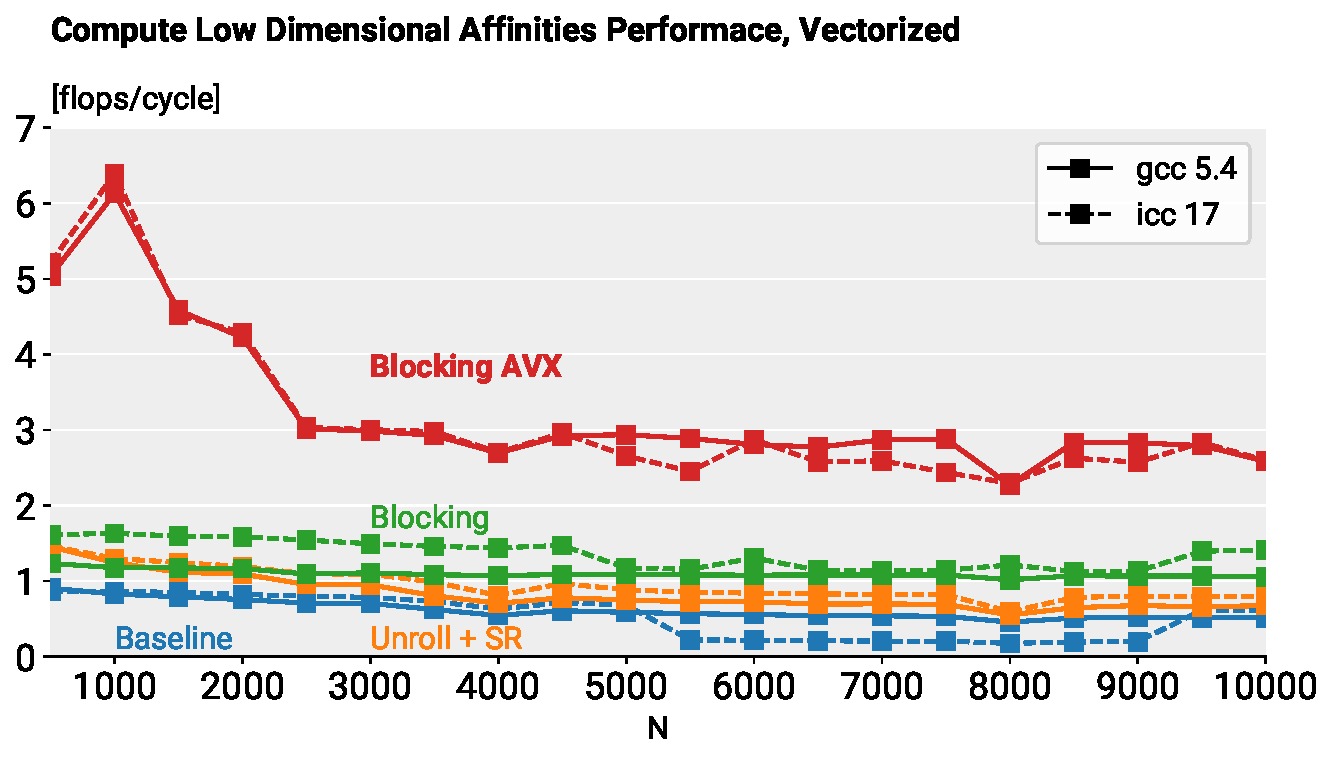
\includegraphics[width=\linewidth]{images/ld_affinities_vec}
  \caption{Performance for the low dimensional affinities. Scalar code was autovectorized. For details about the setup see section~\ref{sec:exp}.}
   \label{fig:bench:ld_affinities}
   \vspace{-5mm}
\end{figure}

\subsubsection{Gradient Computation, Update and Normalize}
Based on the affinities a gradient is computed and the embedding vectors are updated and normalized, to avoid numerical instabilities.
To avoid useless memory access, the gradient is not stored and the points displacement is directly computed. The computation can be seen as $\mathbf{y}_i^{(t)} - \mathbf{y}_i^{(t-1)} = \eta \frac{\partial C}{\partial \mathbf{y}_i^{(t-1)}} + \alpha(t) (\mathbf{y}_i^{(t-1)} - \mathbf{y}_i^{(t-2)}) $ where
$\frac{\partial C}{\partial \mathbf{y}_i^{(t-1)}} = 4 \sum_j (p_{ij} - \frac{t_{ij}}{T}) (\mathbf{y}_i^{(t-1)} - \mathbf{y}_j^{(t-1)}) t_{ij}$.

\mypar{Accumulators}
Unrolling the innermost loop and adding multiple accumulators enabled ILP and boosted the performance close to its ceiling, which is $2.44$ flops/cycle given the instruction mix. In Figure~\ref{fig:bench:gradient} the speedup of this scalar optimization in comparison with the baseline can be seen.

\mypar{Vectorizing}
The next natural step in this optimization is vectorization. The main issue to face is hidden in the sum in the previous equation. Note that the difference of affinities is a scalar, while the difference between points is a 2D vector. However, some effort went into ensuring an optimal computation: loading of the affinities sequentially, perform the computation on them and then transpose the registers with repetition, allowing this to be directly multiplied with the point difference. With this implementation, the performance obtained is around $6$ flops/cycle, a $8.5\times$ speedup compared to the baseline implementation as is plot on Figure~\ref{fig:bench:gradient}.

\mypar{Analysis}
This operation require loading $4N^2 + 2N$ floats and store back $2N$ flops. Since all the gradients are computed at once, and the input size is higher than the cache size, the memory traffic can be defined as $Q(N) \geq 4(4N^2)$. The flop count is $W(N) = 9N^2+3N$, hence we obtain an upper-bound for the operational intensity $I(N) \leq \frac{9}{16} + \mathcal{O}(\frac{1}{N})$.

\begin{figure}[h]
  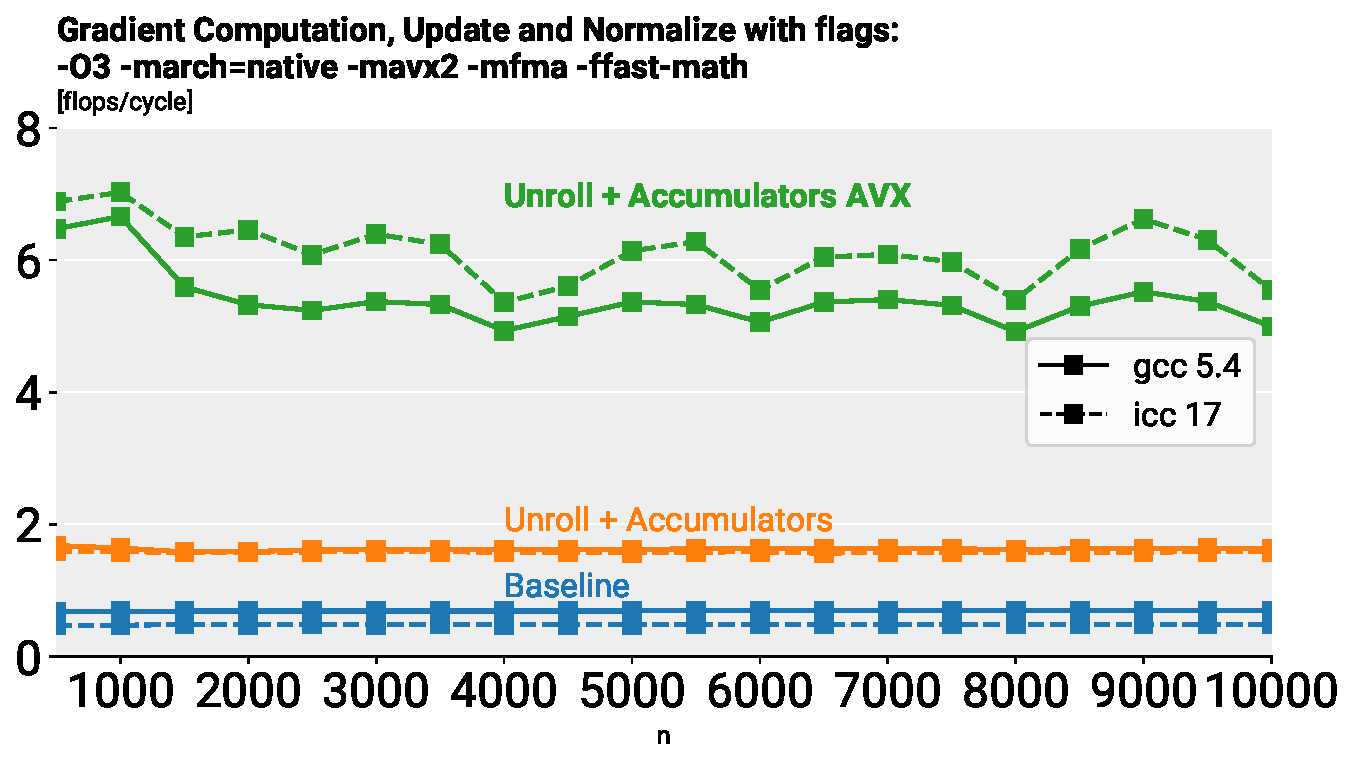
\includegraphics[width=\linewidth]{images/gradient_vec}
  \caption{Performance for the gradient computation. Scalar code was autovectorized. For details about the setup see section~\ref{sec:exp}.}
   \label{fig:bench:gradient}
   \vspace{-5mm}
\end{figure}

\begin{figure}[h]
  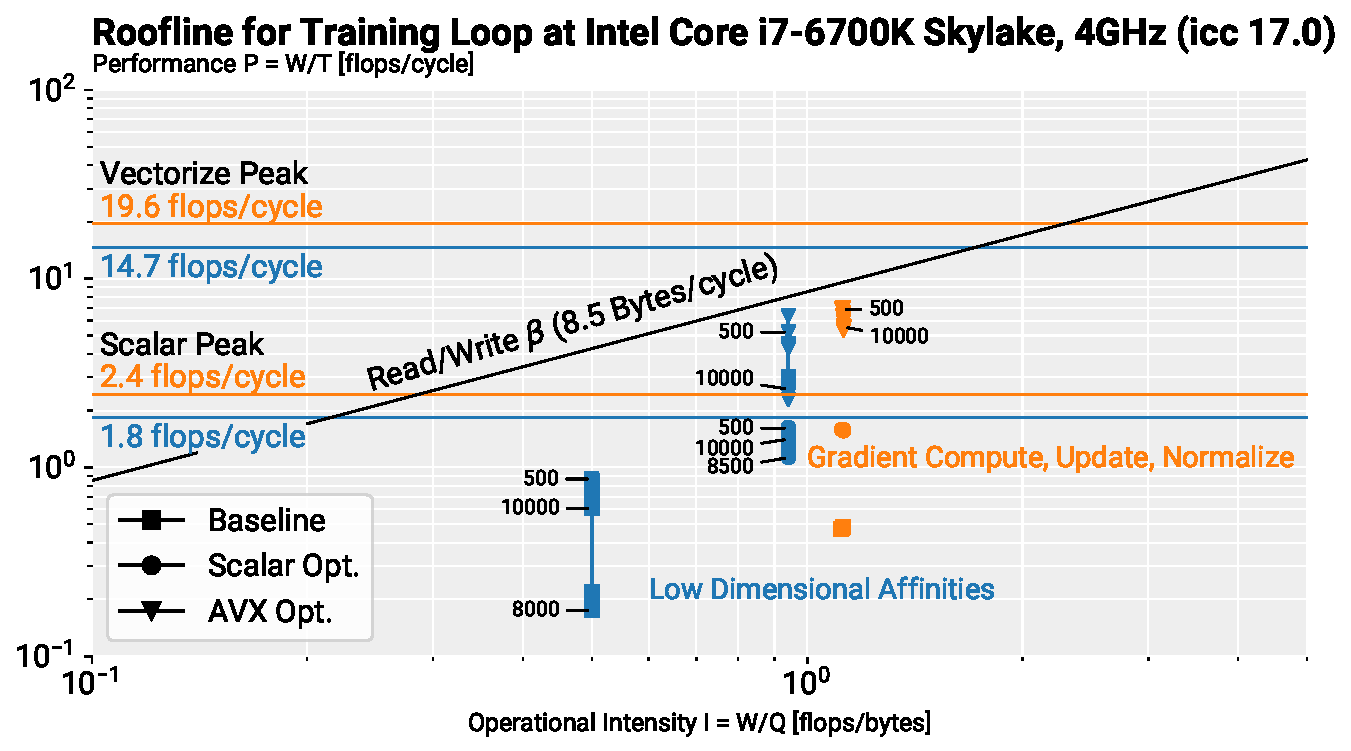
\includegraphics[width=\linewidth]{images/roofline_training_loop}
  \caption{Roofline plot for Part 3.}
   \label{fig:roofline:training}
   \vspace{-5mm}
\end{figure}

Figure~\ref{fig:roofline:training} shows the roofline plot for Part 3. We see that for the scalar case we get close to the theoretical peek, but for the the vectorized case we are ultimately memory bound.

\subsection{Overall Analysis}
Since the parts are independent of each other combining them was straightforward. As almost no data structure fits into cache, we can assume that there is no sharing between parts. This allows us to simply add computations and memory traffic respectively to obtain an OI. As this is a weighted average where Part 3 is weighted with weight $T \approx 1000$, the overall OI is similar to the OI in part 3. Thus the overall roofline is also very similar to the roofline in Figure~\ref{fig:roofline:training}. We confirmed this with Intel Advisor and obtained similar OIs.


\section{Experimental Results}\label{sec:exp}

\mypar{Experimental Setup}
Our benchmarking platform is running Ubuntu 16.04 64-bit and has a Intel Core i7-6700K processor with Skylake architecture and a base frequency of 4 GHz. For our experiments we disabled hyper-threading in the BIOS and disabled turbo boost using \texttt{wrms}. We used \texttt{icc 17} and \texttt{gcc/g++ 5.4}. To benchmark the individual parts we used the benchmarking harness form exercise~2, and for the whole application we used RDTSC.

\begin{sloppypar}
For icc we used the flags \texttt{-O3 -march=core-avx2 -std=c++11 -fp-model fast} and for gcc \texttt{-O3 -march=native -mavx2 -mfma -ffast-math -std=c++11}. When compiling scalar code we also added \texttt{-no-vec} and \texttt{-fno-tree-vectorize -mno-abm} respectively to disable autovectorization.
\end{sloppypar}

The part-wise benchmarks are the median of 11 runs. The total results are the mean of only 3 runs, because running the algorithm for $N > 6000$ is quite expensive.

We used the MNIST dataset\footnote{\url{http://yann.lecun.com/exdb/mnist/}} as it is distributed with the baseline t-SNE implementation. It has input dimension $D=784$.

\begin{figure}[h]
  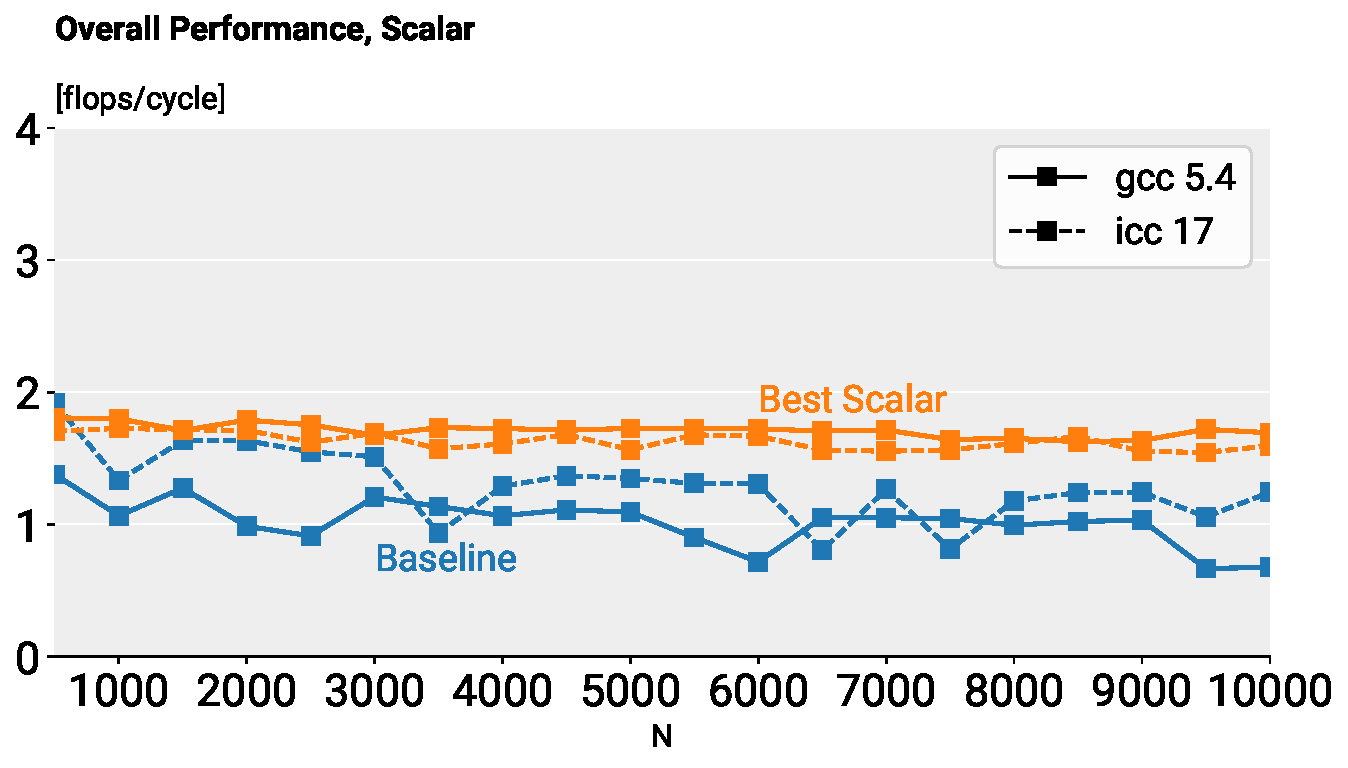
\includegraphics[width=\linewidth]{images/overall_novec}
  \caption{Overall performance, without autovectorization.}
   \label{fig:overall:novec}
      \vspace{-2mm}
\end{figure}

Figure~\ref{fig:overall:novec} shows the performance of our best overall non-vectorized version. We see that for the optimized version the choice of compiler is only a small difference. While for the baseline \texttt{icc} is clearly better. For \texttt{gcc} we get around a $2 \times$ speedup, for \texttt{icc} less.

\begin{figure}[h]
  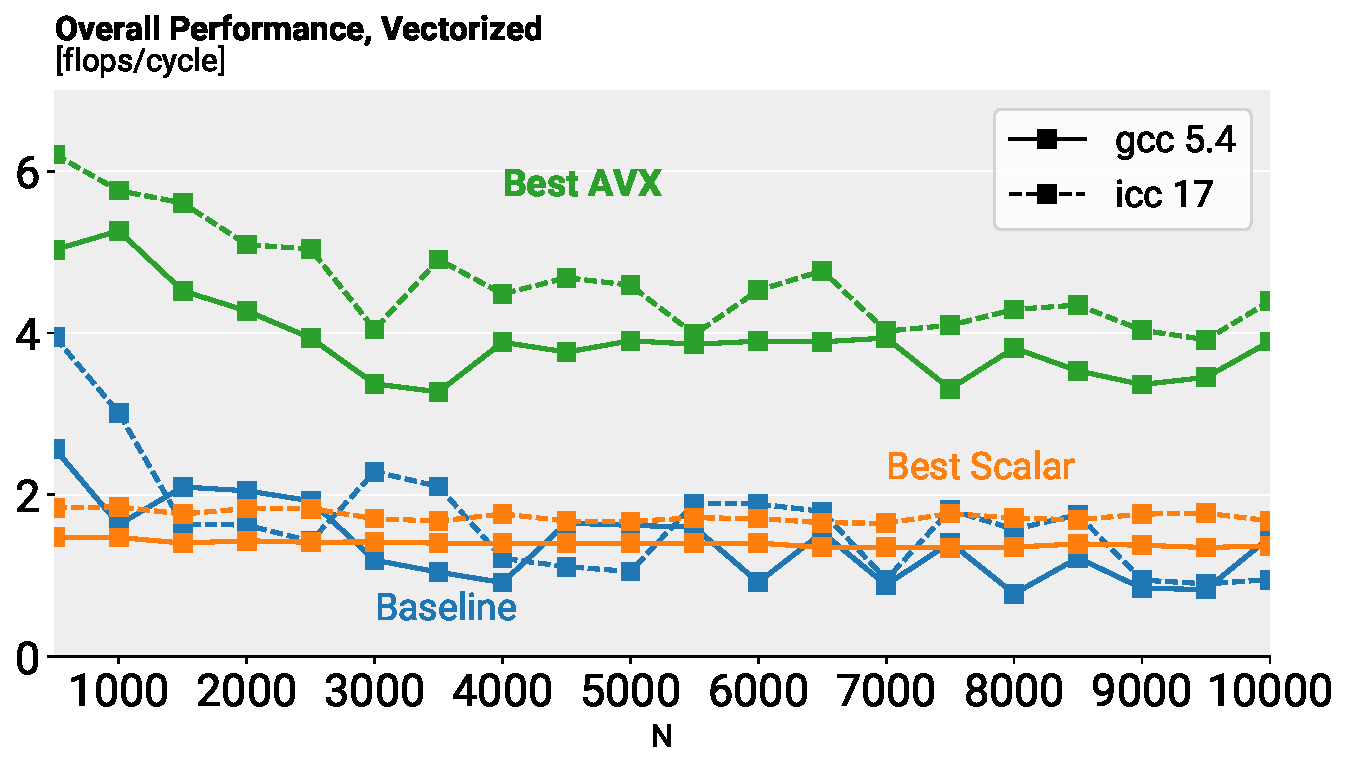
\includegraphics[width=\linewidth]{images/overall_vec}
  \caption{Overall performance, scalar code autovectorized.}
   \label{fig:overall:vec}
      \vspace{-2mm}
\end{figure}

Figure~\ref{fig:overall:vec} shows the best vectorized results. With autovectorization enabled the baseline becomes actually comparable to the to the fast scalar version. Both are around 2 flops/cycle. While the hand-vectorized code has around 4 flops/cycle.
It seems auto-in-lining the baseline implementation and then applying autovectorization produces a decent vectorized version in both \texttt{gcc} and \texttt{icc}.

Before any optimization $7.79 \%$ of cycles are spend in Part 1, $3.86 \%$ in Part 2 and $88.35 \%$ Part 3. In the final version $2.44 \%$ in Part 1, $2.47 \%$ in Part 2 and $95.11 \%$ in Part 3. The values are averaged over all input sizes. This shows that Part 3 remains the bottleneck. Since Part 3 is dominant with $90 \%$ we can assume that it's performance ceiling applies to the whole. Since the time is spend about the same in both steps of Part 3, we can average them. This gives us a theoretical peek performance of $2.14$ flops/cycles for the scalar case. Thus we obtain around $80-90 \%$ of the theoretical peak performance, which is about $40-50\%$ of the platform peak of $4$ flops/cycle. In the vectorized case similar analysis shows that we have around $25-30\%$ of the theoretical peak, which is around $12 \%$ of the machine peek of $32$ flops/cycle. As the roofline plot in Figure~\ref{fig:roofline:training} shows, we are ultimately memory bound in the most important part of the computation.


\section{Conclusions}

We showed a roughly 2-4x speedup for the best known implementation of the $N^2$ t-SNE algorithm. For the scalar case this is close to the theoretical peek performance, while in the vectorized version we are more strongly memory bound. Optimizations like the squared euclidean distance, specialized for $d=2$ and very high dimensions, can be easily applied to other machine learning algorithms, as is a very common pattern. In order to handle large numbers of inputs $N$, applying the already considered optimizations to the $N \log N$ version seems the next logical step. Another direction would be to generalizing part 3 to output dimensions other than 2. One could imagine to hand-craft the important cases $d=2$ and $d=3$ and use generic code or code generation for other numbers of output dimensions.


% References should be produced using the bibtex program from suitable
% BiBTeX files (here: bibl_conf). The IEEEbib.bst bibliography
% style file from IEEE produces unsorted bibliography list.
% -------------------------------------------------------------------------
\bibliographystyle{IEEEbib}
\bibliography{bibl_conf}

\end{document}
